%-----------------------------------------------------------------------------%
\chapter{\babTiga}
%-----------------------------------------------------------------------------%
%\todo{tambahkan kata-kata pengantar bab 1 disini}

%-----------------------------------------------------------------------------%
\section{Studi Literatur}
%-----------------------------------------------------------------------------%

\section{Analisis}

Analisis dilakukan untuk mengkaji masalah yang ada, mendefinisikan
batasan dalam masalah, lalu mencari solusi dari masalah tersebut. Analisis juga
meliputi performa rancangan modul yang telah diberi watermark yang diuji coba
dalam board FPGA.

\section{Perancangan}

Pada tahap ini dilakukan pengkajian masalah serta pendefinisian batasan
masalah. Pencarian solusi atas masalah yang muncul juga dilakukan. Tahap ini
juga meliputi analisis penempatan dan penentuan jalur dalam pemasangan
rangkaian uji IP Protection pada VLSI.

\begin{figure}[h]
	\centering
	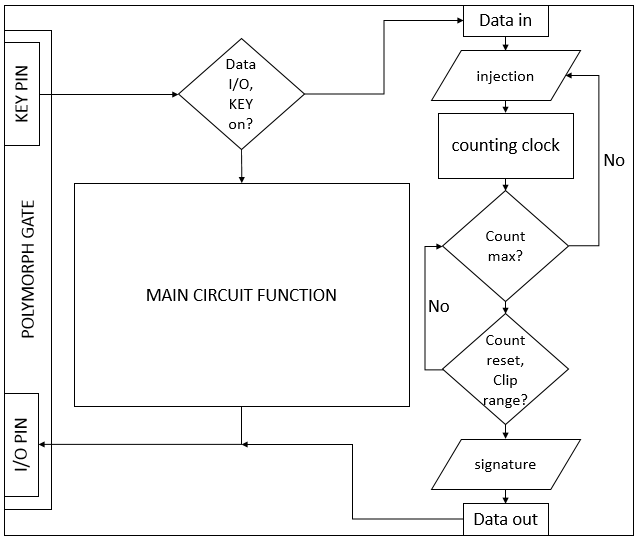
\includegraphics[scale=0.6]{images/flow}
	\caption{Simulation results for the network.}
	\label{fig_sim}
\end{figure}

\begin{figure}[h]
	\centering
	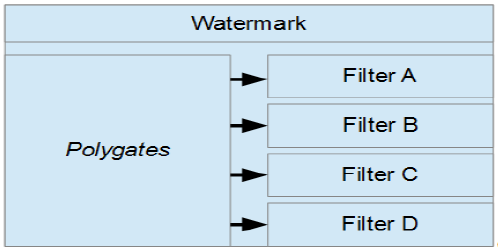
\includegraphics[scale=0.8]{images/box}
	\caption{Simulation results for the network.}
	\label{fig_sim}
\end{figure}

Penelitian kali ini akan melakukan simulasi desain controller HDMI
menggunakan FPGA. Desain controller ini akan di-tes performa-nya dengan
menjalankan fail multimedia. Controller akan disambung-kan ke connector
HDMI lalu menampilkan hasil keluaran multimedia pada monitor atau TV.
Kemudian di dalam controller HDMI ini akan disisipkan rangkaian watermark
dan akan dilakukan pengecekan performa-nya lagi untuk mengetahui terjadinya
penurunan performa karena watermark.

% Table generated by Excel2LaTeX from sheet 'Data encripted'
\begin{table}[htbp]
	\centering
	\caption{Add caption}
	\begin{tabular}{rlll}
		\cline{2-3}    \multicolumn{1}{r|}{} & \multicolumn{1}{c|}{Alphabet} & \multicolumn{1}{c|}{Biner} &  \bigstrut\\
		\cline{2-3}    \multicolumn{1}{r|}{} & \multicolumn{1}{c|}{H} & \multicolumn{1}{c|}{111} &  \bigstrut\\
		\cline{2-3}    \multicolumn{1}{r|}{} & \multicolumn{1}{c|}{F} & \multicolumn{1}{c|}{101} &  \bigstrut\\
		\cline{2-3}    \multicolumn{1}{r|}{} & \multicolumn{1}{c|}{G} & \multicolumn{1}{c|}{110} &  \bigstrut\\
		\cline{2-3}    \multicolumn{1}{r|}{} & \multicolumn{1}{c|}{C} & \multicolumn{1}{c|}{010} &  \bigstrut\\
		\cline{2-3}    \multicolumn{1}{r|}{} & \multicolumn{1}{c|}{D} & \multicolumn{1}{c|}{011} &  \bigstrut\\
		\cline{2-3}    \multicolumn{1}{r|}{} & \multicolumn{1}{c|}{E} & \multicolumn{1}{c|}{100} &  \bigstrut\\
		\cline{2-3}    \multicolumn{1}{r|}{} & \multicolumn{1}{c|}{C} & \multicolumn{1}{c|}{010} &  \bigstrut\\
		\cline{2-3}    \multicolumn{1}{r|}{} & \multicolumn{1}{c|}{A} & \multicolumn{1}{c|}{000} &  \bigstrut\\
		\cline{2-3}    \multicolumn{1}{r|}{} & \multicolumn{1}{c|}{H} & \multicolumn{1}{c|}{111} &  \bigstrut\\
		\cline{2-3}    \multicolumn{1}{r|}{} & \multicolumn{1}{c|}{E} & \multicolumn{1}{c|}{100} &  \bigstrut\\
		\cline{2-3}    \multicolumn{1}{r|}{} & \multicolumn{1}{c|}{C} & \multicolumn{1}{c|}{010} &  \bigstrut\\
		\cline{2-3}    \multicolumn{1}{r|}{} & \multicolumn{1}{c|}{B} & \multicolumn{1}{c|}{001} &  \bigstrut\\
		\cline{2-3}    \multicolumn{1}{r|}{} & \multicolumn{1}{c|}{C} & \multicolumn{1}{c|}{010} &  \bigstrut\\
		\cline{2-3}    \multicolumn{1}{r|}{} & \multicolumn{1}{c|}{F} & \multicolumn{1}{c|}{101} &  \bigstrut\\
		\cline{2-3}    \multicolumn{1}{r|}{} & \multicolumn{1}{c|}{D} & \multicolumn{1}{c|}{011} &  \bigstrut\\
		\cline{2-3}    \multicolumn{1}{r|}{} & \multicolumn{1}{c|}{E} & \multicolumn{1}{c|}{100} &  \bigstrut\\
		\cline{2-3}    \multicolumn{1}{r|}{} & \multicolumn{1}{c|}{C} & \multicolumn{1}{c|}{010} &  \bigstrut\\
		\cline{2-3}    \multicolumn{1}{r|}{} & \multicolumn{1}{c|}{H} & \multicolumn{1}{c|}{111} &  \bigstrut\\
		\cline{2-3}    \multicolumn{1}{r|}{} & \multicolumn{1}{c|}{D} & \multicolumn{1}{c|}{011} &  \bigstrut\\
		\cline{2-3}          &       &       &  \bigstrut[t]\\
		INPUT : & \multicolumn{3}{l}{HFGCDECAHECBCFDECHD} \\
		OUTPUT : & \multicolumn{3}{l}{CABE} \\
	\end{tabular}%
	\label{tab:addlabel}%
\end{table}%



Dalam penelitian ini teknik watermark yang digunakan adalah
menggabungkan rangkaian logical polimorph gate sebagai kunci utama untuk
mengaktifkan rangkaian Digital Signal Filter yang akan diberi masukan kunci
kedua untuk memanggil data watermark dalam chip.

\begin{figure}[!h]
	\centering
	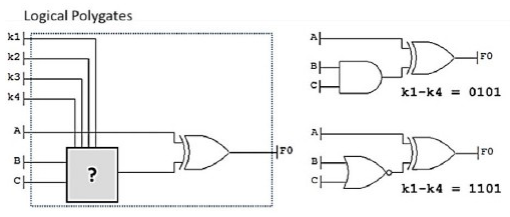
\includegraphics[scale=0.8]{images/polymorphgate}
	\caption{Simulation results for the network.}
	\label{fig_sim}
\end{figure}

Setelah unique key dari Polygates di masukan (contoh: K1 - K4), maka pin
input untuk algoritme DSP aktif (contoh: pin A – C) yang kemudian akan
mengolah key untuk penampilan watermark dalam chip.

Setelah polygate mengaktifkan filter yang dipilih maka data dari pin input
DSP (contoh: pin A – C) masuk ke dalam filter yang aktif dan akan diolah sebagai
data input watermark.

\section{Pengujian}

Pada tahap ini dilakukan serangkaikan uji coba untuk mengukur parameter
performa rangkaian VLSI yang telah disisipkan rangkaian uji IP Protection.
Petitcolas [13] mengidentifikasi beberapa hal yang menjadi bahan evaluasi untuk
IP Protection :

\subsection{Kerahasiaan algoritme}

Merujuk pada aturan keamanan yang dijelaskan oleh Kerckhoffs [14] pada
tahun 1883, setiap enkripsi atau teknik keamanan tidak boleh mengandalkan
kerahasiaan suatu algoritme, tetapi pada kompleksitas matematis algoritme
tersebut.

\subsection{Tingkat Ketahanan Uji}

Ini adalah aspek yang sangat penting. Aspek ini berisi tentang ketahanan
algoritme dari serangan dan persentase dari IP Protection tak terdeteksi.
Kemungkinan detector salah mendeteksi algoritme pada rangkaian tanpa
algoritme juga diperhitungkan di aspek ini.

\begin{figure}[!h]
	\centering
	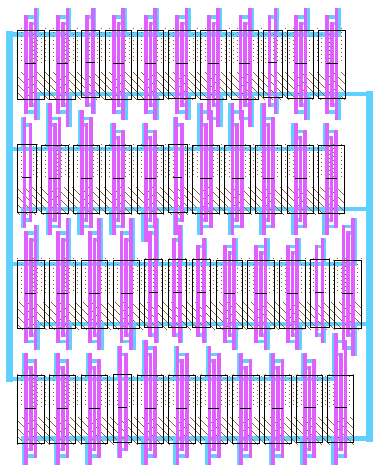
\includegraphics[scale=0.8]{images/gate1}
	\caption{Simulation results for the network.}
	\label{fig_sim}
\end{figure}

\begin{figure}[!h]
	\centering
	
\includegraphics[scale=0.8]{images/gatePlace}
	\caption{Simulation results for the network.}
	\label{fig_sim}
\end{figure}

\subsection{Tingkat Penurunan Performa}

Penurunan performa saat menyisipkan suatu metode IP Protection adalah
hal yang tak dapat dihindari. Tetapi penurunan performa yang terlalu besar akan
menjadi masalah. Maka dari itu, perbandingan performa antara rangkaian yang
telah disisipkan IP Protection dan rangkaian tanpa IP Protection harus dilakukan.

\subsection{Tingkat Deteksi}

Penyisipan watermark merupakan bagian dari proses, pelacak-kan dan
deteksi dalam teknik watermark IC. Pelacak-kan dan deteksi watermark pada
kemungkinan penyerangan merupakan aspek yang akan dijadikan pertimbangan
pada teknik watermark.

\section{Data Pengujian}

Metode yang akan digunakan merupakan simulasi pada board FPGA
dengan desain modul yang sudah ada dan menyisipkan suatu rangkaian tambahan
watermarking dan menguji perubahan performa modul yang telah di sisipkan
watermark tersebut.

Dalam penelitian ini akan menggunakan teknik Digital Signal Processing
Watermarking pada modul yang telah ada dengan kombinasi perhitungan loop
biner dengan output yang akan membentuk nama dari produsen asli modul
tersebut. Modul yang telah diberi watermark akan tetap dapat diuji keabsahan
pemiliknya walaupun modul telah digabungkan dengan modul lain dalam sebuah
proyek modul VLSI.

Kemudian setelah modul disisipkan watermark, kami akan menguji
performa modul tersebut dengan mengharapkan tidak ada perubahan berarti
terhadap modul yang telah diberi watermark tersebut.
